\chapter{INTRODUCTION}


What happens to an atom in an electric field? An atom is a neutral particle so it will not accelerate in a uniform electric field, however, it is composed of positively charged protons and negatively charged electrons that do feel electric forces. If we place our test atom in a charged parallel-plate capacitor, the negatively charged electrons tend to move toward the positively charged surface, while the much heavier and positively charged nucleus moves only slightly toward the negatively charged surface. As a result of these movements, the atom becomes stretched out by an amount determined by its \emph{polarizability}. Figure \ref{simplePolFig} shows a cartoon of this idea. The polarizability of a spherical particle is proportional to its volume and this remains approximately true for atoms as well. As such, polarizability is conveniently expressed in terms of a volume, typically $a_0^3$ or 10$^{-24}$ cm$^3$. The SI unit of polarizability, C m$^2$/V, can be reduced to a volume by simply dividing by $4\pi\epsilon_0$. 


\begin{figure}
\centerline{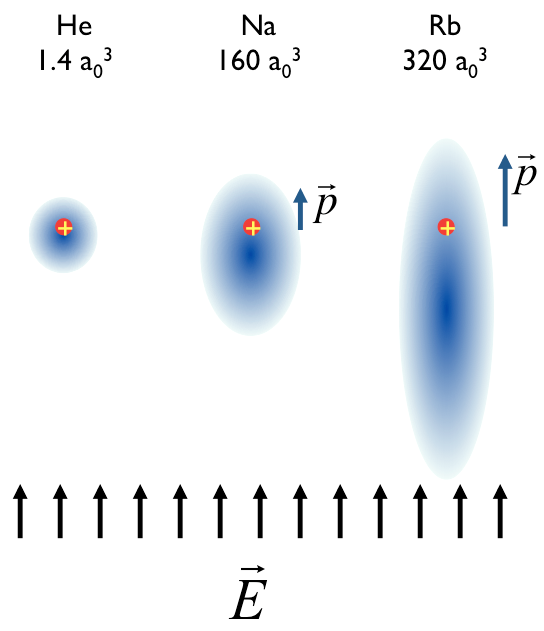
\includegraphics[width=0.5\textwidth]{Figures/simplePolFigv2.png}}
\caption[An electric field applied to an atom induces a dipole moment in proportion to its atomic polarizability.]{\label{simplePolFig}An electric field applied to three different atoms, helium, sodium, and rubidium, induces a dipole moment in proportion to the atomic polarizability. The polarizability roughly scales in proportion to the volume of the atom.}
\end{figure}


More precisely, the polarizability $\alpha$ of an atom relates the induced dipole moment $\vec{p}$ to the applied electric field $\vec{E}$ by
\begin{eqnarray}
\vec{p} = \alpha \vec{E} +  ...
\end{eqnarray}
The dipole moment is $\vec{p}=e\vec{r}$, where $\vec{r}$ is the displacement of the electron cloud. Higher order terms, such as the hyperpolarizability, will be neglected in this work since we operate our experiments at more than $10^5$ times below the scale of the atomic field ($\vec{E}_a \approx e/a_0^2=5\times10^{11}$ V/m). 


The energy shift of a polarizable particle in an electric field is given by
\begin{eqnarray}
\label{starkShift}
U = -\frac{1}{2} \alpha \vec{E}^2,
\end{eqnarray}
and this is commonly referred to as the Stark shift. Polarizability can also be defined through 2nd-order perturbation theory. The Hamiltonian of a polarizable particle is
\begin{eqnarray}
H = H_\textrm{atom} - \hat{p} \cdot \vec{E}
\end{eqnarray}
where $\hat{p}$ is the dipole operator. Application of 2nd order perturbation theory leads to a ground-state static polarizability of
\begin{eqnarray}
\label{pertubationTheoryEqn}
\alpha = 2e^2 \sum_{i\neq0} \frac{ | \langle i | \vec{r} . \vec{E} | 0 \rangle |^2}{E_i}
\end{eqnarray}
where $e$ is the electron charge and $E_i$ is the energy of the $i$th atomic state, assuming $E_0 \equiv 0$. So far we have assumed that the applied field is constant in time, but we will examine the frequency dependence of the dynamic polarizability in sections \ref{mzwBrief} and \ref{dynPolSec}.


Equation \ref{pertubationTheoryEqn} gives us insight into why polarizability is an interesting property to study: it can be expressed as a sum of dipole matrix elements. These matrix elements also describe properties such as transition strengths, state lifetimes, van der Waals interactions, indices of refraction, and scattering cross-sections, just to name a few. In fact, in a 1966 review of atomic polarizabilities, Bederson and Robinson referred to polarizability as a ``seemingly ubiquitous parameter" \cite{Bed66} and T.M.~Miller compiled a list of properties directly related to polarizability with more than 15 entries \cite{Mil12}. Since dipole matrix elements are notoriously difficult to calculate, experiments such as the ones described in this thesis can serve as input to a long list of calculations.


New applications of atomic physics continue to demand better knowledge of atomic polarizabilities. Next generation optical lattice clocks based on strontium and ytterbium atoms suffer from significant frequency shifts due to blackbody radiation and accurate calibration of these frequency shifts requires precise knowledge of polarizabilities \cite{Lud08,Der11}. Parity non-conservation studies \cite{Woo97,Tsi09} using atomic systems impose limits on physics beyond the standard model, but require accurate atomic structure calculations to interpret the measurements \cite{Der07}. Polarizability measurements are some of the best ways to test these calculations.


This thesis describes three experiments all concerned with precisely answering the seemingly simple question of what happens to an atom in an electric field. The most important findings are as follows:
\begin{itemize}
\item I used an atom interferometer and a novel electric field gradient geometry to measure the polarizabilities of K and Rb with unprecedented precision (0.5\% uncertainty) \cite{Hol10}. These measurements are now listed in the CRC Handbook of Chemistry and Physics, and they establish a roadmap for future polarizability measurements in our lab.
\item I developed a new technique to measure atom beam velocities with 0.1\% uncertainty using phase choppers \cite{Hol11}. This technique will enable more precise polarizability measurements.
\item I measured a wavelength, referred to as a magic-zero wavelength, for which the dynamic polarizability of potassium equals zero. We measured the first, i.e.~the longest, magic-zero wavelength of potassium with 1.5 pm uncertainty \cite{Hol12a}. I explain how this is a novel method to test atomic structure calculations and also establishes a foundation for future measurements of magic-zero wavelengths in our lab.
\end{itemize}



The remainder of this introduction provides a brief history of polarizability measurements and a review of the basic matterwave optics needed for understanding the experiments in this thesis. Chapter 2 summarizes the experiments, papers, and proposals that comprise this thesis work. Chapters 3-5 provide supporting material for our peer-reviewed publications on static polarizability measurements of Na, K, and Rb (Appendix A) \cite{Hol10}, a new atom velocity measurement technique using phase choppers that will improve polarizability measurements (Appendix B) \cite{Hol11}, and a measurement of the first magic-zero wavelength of the dynamic polarizability of potassium (Appendix C) \cite{Hol12a}. Chapters 6 and 7 propose two new experiments: measurements of Sr polarizability using a resonant photoionization detector and measurements of the tensor polarizabilities of alkali dimers.








%%%%%%%%%%%%%%%%%%%%%%%%%%%%%%%%%%%%%
\section{A brief history of polarizability measurements}
\label{introPolHistory}
In this section we provide a brief review of the history of polarizability measurements. For comprehensive reviews of polarizability measurements, see Mitroy, Safronova and Clark (2010) \cite{Mit10}, Gould and Miller (2005) \cite{Gou05}, Hohm (2000) \cite{Hoh00}, Miller and Bederson (1989) \cite{Mil89}, Miller and Bederson (1978) \cite{Mil78}, Bederson and Robinson (1966) \cite{Bed66}, and the CRC Handbook of Chemistry and Physics \cite{Mil12}. 

Scheffers and Stark started the business of polarizability measurements in 1934 \cite{Sch34} by deflecting atomic beams of Li, K, and Cs in an inhomogenous electric field. More than 25 years later, Benjamin Bederson developed the E-H gradient spectrometer at NYU \cite{Bed60} and in 1961 made the first measurements of polarizabilities since Stark \cite{Sal61}. These measurements were made with about 15\% uncertainty and formed the foundation for a career's worth of impressive polarizability measurements discussed below. 

In 1974, \emph{Physical Review A} published two landmark polarizability measurement papers. Hall and Zorn \cite{Hal74} measured the polarizabilities of the alkalis Na through Cs with 7\% uncertainty using beam deflection, and Molof, Schwartz, Miller, and Bederson \cite{Mol74} measured the polarizabilities of Li through Cs and the $^3\textrm{P}_2$ metastable nobel gas atoms with 2\% uncertainty using the E-H gradient balance technique. Molof \etal provided measurements of polarizability unmatched for over 2 decades and has been cited over 200 times. Molof \etal achieved their relatively low uncertainties by measuring polarizabilities with respect to the polarizability of metastable He, which can be calculated with high precision. In this thesis, we continue the technique of using ratio measurements of polarizabilities for improved precision.

The Bederson group also measured the average dipole polarizabilities of homonuclear alkali dimers with 10\% uncertainty in 1974 by using ratios with respect to the polarizabilities of the alkali atoms \cite{Mol74a}. The polarizabilities of Ba, Sr \cite{Sch74} and Ca \cite{Mil76} were also measured with respect to Li over the next two years. In 1993, Tarnovsky \etal measured the polarizabilities of both the homonuclear and heteronuclear alkali dimers with Bederson \cite{Tar93}. These measurements were made with 6-10\% uncertainty.

The 1990s saw the advent of atom interferometry and its promise of high precision measurements of atomic properties \cite{Eks95, Mif06, Lep11a}, fundamental constants of nature \cite{Fix07}, and inertial displacements \cite{Len97, Gus97}. The Pritchard group at MIT made the first interferometry-based precision polarizability measurement of an atom, Na, with 0.35\% uncertainty using a three nanograting Mach-Zehnder atom interferometer \cite{Eks95}. In Toulouse, the Vigu\'{e} group measured the polarizability of Li with 0.66\% uncertainty using an atom beam interferometer with light gratings \cite{Mif06}. The Arndt group in Vienna measured the polarizability of $C_{60}$ and $C_{70}$ with 6\% uncertainty and their ratio with 2.5\% uncertainty using a near field interferometer \cite{Ber07}. 

The development of laser trapping and cooling enabled several new polarizability measurements, as well. The Sackett group in Virginia measured the dynamic polarizability of Rb near the D1 and D2 lines with 7\% uncertainty using a guided ultracold atom interferometer \cite{Dei08}. Amini and Gould used an atomic fountain to measure the polarizability of Cs with 0.14\% uncertainty \cite{Ami03}. This measurement provides a valuable benchmark for calculations \cite{Der07, Por09} needed to interpret atomic parity non-conservation experiments \cite{Woo97}. Cold atom experiments offer much longer interaction times than atom beam experiments and ultracold atom interferometers may offer better than shot-noise limited precision. However, these experiments often suffer from additional systematic errors, such as density-dependent phase shifts, and therefore independent measurements provide valuable cross-checks. 

Other notable measurements of polarizabilities of non-alkali or alkaline-earth atoms include the following. Sch\"{a}fer \etal measured the polarizability of lead clusters using beam deflection \cite{Sch08}. The Bederson group also made measurements of the polarizability of mercury \cite{Lev68}, indium \cite{Gue84}, and the alkali halide dimers \cite{Gue91}. Knight \etal measured the polarizability of sodium clusters \cite{Kni85}. The Kresin group at UCLA measured the polarizability of sodium clusters \cite{Tik01} using 
electrodes from the Bederson group. These measurements all have uncertainties on the order of a few percent.

Mitroy, Safronova, and Clark recently wrote a comprehensive review of the theory of atomic polarizabilities with extensive references \cite{Mit10}. In addition, I recommend references \cite{Dal62,Rei76,Mul84,Der99,Saf99,Lim05atoms,Saf06} to trace the progress of polarizability calculation techniques through the past half-century. 

I provide a recommendation for the best measurements and calculations of polarizability of the alkali atoms in Table \ref{polResultsRecValues}. The theoretical uncertainty of polarizability for most alkalis is about 0.1\%, while the measurement uncertainty is 0.2-0.5\%. Note that our measurements of potassium and rubidium polarizability presented in this thesis are the best available. 

Techniques developed in this thesis, specifically the use of ratio measurements of polarizability and the ability to measure the polarizability of heavy atoms using an atom beam interferometer, will enable measurements of alkali atom polarizabilities with better than 0.1\% uncertainty. As I explain in Chapter \ref{polChapter} and Appendix B, we have demonstrated measurements of cesium polarizability with a precision of 0.1\%, but not yet this accuracy. 


\begin{table}
\caption[Recommended measured and calculated values of alkali static polarizabilities.]{\label{polResultsRecValues}Recommended measured and calculated values of alkali static polarizabilities in units of $10^{-24}\textrm{ cm}^3$. Some calculations rely on measurements of atomic properties. See Mitroy \etal \cite{Mit10} for more details.}
\begin{center}
\begin{tabular}{l l l }
\hline\hline
Atom & $\alpha_\textrm{meas}$ & $\alpha_\textrm{calc}$ \\
\hline
Li & 24.33(16) \cite{Mif06} & 24.318(4) \cite{Tan10} \\
Na & 24.11(8) \, \cite{Eks95} & 24.09(4)\,\,\, \cite{Der99} \\
K & 43.06(21) \cite{Hol10} & 42.91(9) \, \cite{Aro07} \\
Rb & 47.24(21) \cite{Hol10} & 47.17(9) \, \cite{Aro12a} \\
Cs & 59.42(8) \, \cite{Ami03} & 59.26(3) \, \cite{Der99}  \\
\hline
\end{tabular}
\end{center}
\end{table}






%%%%%%%%%%%%%%%%%%%%%%%%%%%%%%%%%%%%%%
\section{Matterwave optics}
\label{matterwaveOptics}
Matterwave optics and atom interferometry is now a mature tool that has been extensively described in numerous reviews \cite{Ram56,Ber97,Mif06a,Cro09,Hor12}, primary references \cite{Kei91,And97,Bre02,Wan05,Gar06,Hof06,Ger07,Chi11}, and Ph.D.~theses \cite{Kok01,Rob02,Per05Thesis,McM09,Lon11a}. Here, I summarize only the essential principles of our particular atom interferometer to provide background for the measurements described later in this thesis.


Our atom beam is created by supersonic expansion \cite{Hab85, Sco88} of an inert carrier gas seeded with alkali atoms and collimated with two small slits. A translatable hot-wire detector \cite{Del02RSI} and channel electron multiplier measures the atom beam flux. See V.P.A. Lonij's thesis, section 2.2, for more details of our updated atom beam source and detector \cite{Lon11a}.


A silicon-nitride nanograting diffracts the collimated atom beam, just as a traditional grating will diffract light waves. The path separation after the first grating is 
\begin{eqnarray}
\label{sepEqn}
s=\frac{\lambda_{dB}}{d_g}z=\frac{h}{mvd_g}z
\end{eqnarray}
where $\lambda_{dB}=h/mv$ is the de Broglie wavelength of an atom with mass $m$ and velocity $v$, $d_g=100$ nm is the grating period, and $z$ is the propagation distance from the first grating. For typical beam conditions in our experiments $\lambda_{dB}\approx5$ pm, and this results in a diffraction angle of 50 $\mu$rad. Lonij \etal \cite{Lon09,Lon10} and Perreault \etal \cite{Per05pra} used atom beam diffraction to study atom surface interactions. 


We use a three-grating Mach-Zehnder atom interferometer (Figure \ref{simpleIFM}) to make precision measurements of atomic properties. This interferometer is an evolution of the machine developed in Dave Pritchard's group at MIT in the 1980s and 1990s \cite{Kei91,Ber97,Kok01}. A superposition of two traveling waves, created by diffraction from the first and second nanogratings, forms a sinusoidal interference pattern in space at the plane of the third nanograting. These two traveling waves may be written as 
\begin{eqnarray}
\psi_{0}&=&Ae^{i(k_z z + \phi_0)}\\
\psi_{1}&=&Be^{i(k_z z + k_x x + \phi_1)}.
\end{eqnarray}
The transverse wavenumber is determined by the period of the nanogratings: $k_x=2\pi/d_g$. 


\begin{figure}
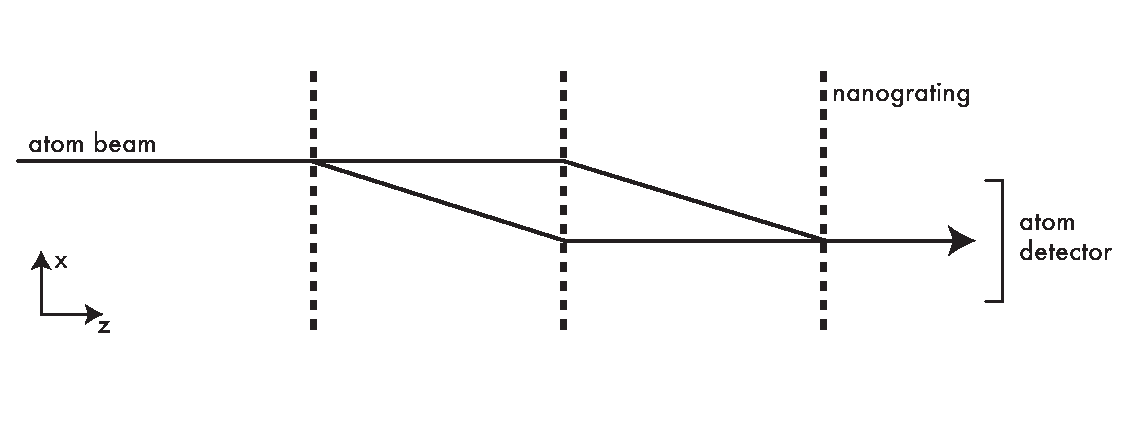
\includegraphics[width=1\textwidth]{Figures/bareIFM.eps}
\caption[A three grating Mach-Zehnder atom interferometer.]{\label{simpleIFM}A three grating Mach-Zehnder atom interferometer. Atoms waves diffracted by the first and second nanogratings form an interference pattern at the third nanograting. A hot-wire detector measures the transmitted atom beam flux.}
\end{figure}


The superposition of traveling waves overlaps at the location of the 3rd nanograting and make a probability of detecting each atom at location $x$ given by
\begin{eqnarray}
|\psi|^2&=&|\psi_0+\psi_1|^2\nonumber\\
&=&A^2+B^2+AB\left(e^{i(k_x x + \delta_\phi)}+e^{-i(k_x x + \delta_\phi)}\right)\nonumber\\
&=&A^2+B^2+2AB\cos(k_x x + \delta_\phi)
\end{eqnarray}
where $\delta_\phi = \phi_1-\phi_0$. The probability density is described by a constant value plus a term that oscillates with a spatial frequency equal to the nanograting period, regardless of the atomic velocity $v=\hbar k_z/m$. As such, we can use a 3rd nanograting as a mask of the interference pattern. The transmitted flux, $I(x)$, can be written in terms of an average beam flux $I_0$, contrast $C$, and phase $\delta_\phi$:
\begin{eqnarray}
I(x)=I_0+C\cos(k_x x + \delta_\phi).
\end{eqnarray}
Moving any of the nanogratings in the $x$ direction scans the atomic interference pattern across the third nanograting to yield intensity vs.~position data. A co-propogating laser interferometer measures the relative position of the three nanogratings. Figure \ref{atomFringe} shows an example of the atom interference fringe data. 


The observed fringe pattern is the incoherent sum of the sinusoidal probability distributions from single-atom interference, repeated about $10^5$ times per second. Different atoms have different velocities and also enter and exit the interferometer at different times. Atoms do not interfere with other atoms in our interferometer, only with themselves, because they are separated from other atoms by tens of micrometers on average. These characteristics are crucial for understanding contrast loss in our interferometer, and in particular the new velocity measurement technique described in section \ref{choppersBrief} and Appendix B. 


Application of, say, an electric field gradient across the interferometer changes $\delta_\phi$ and results in a measurable phase shift. We analyze these phase shifts to determine properties such as atomic polarizability, described in section \ref{polBrief} and Appendix A, and magic-zero wavelengths, described in section \ref{mzwBrief} and Appendix C.


\begin{figure}
\centerline{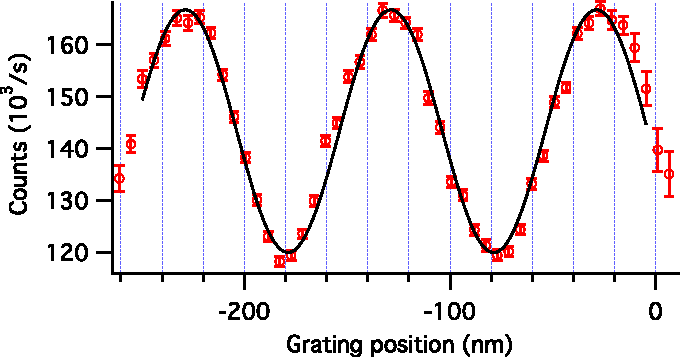
\includegraphics[width=.75\textwidth]{Figures/atomFringe.pdf}}
\caption[Atom interference fringe.]{\label{atomFringe}A typical atom interference fringe from our Mach-Zehnder atom interferometer determined from 5 sec of data. We fit this data to find the fringe contrast $C$ and phase $\phi$.}
\end{figure}


The phase of the atom waves along each path evolve according to
\begin{eqnarray}
\phi=\frac{1}{\hbar} \int E(t) dt
\end{eqnarray}
where $E(t)$ is the total energy of the atom as a function of time. All of the phase shifts described in this thesis are created by energy shifts ($\sim$1 $\mu$eV) much smaller than the kinetic energy of the atoms ($\sim$0.1 eV), and much more slowly varying ($\sim$100 $\mu$m) than the de Broglie wavelength ($\sim$10 pm). These are, loosely, the conditions for the application of the WKB approximation. In the WKB approximation the phase is described by
\begin{eqnarray}
\phi=\frac{1}{\hbar} \int p(z) dz
\end{eqnarray}
where
\begin{eqnarray}
p(z) = \sqrt{2m(E-U(z))}
\end{eqnarray}
is the momentum of the atom. Since $U(z)\ll E$ we can simplify the phase:
\begin{eqnarray}
\phi &=& \frac{\sqrt{2mE}}{\hbar} \int \sqrt{1-\frac{U(z)}{E}} dz \\
	&\approx& \frac{\sqrt{2mE}}{\hbar} \int \left(1-\frac{U(z)}{2E} \right) dz.
\end{eqnarray}
The first term will be common to both paths and not measurable, so we drop it from consideration. The second term corresponds to the change in phase of the wavefunction due to the application of a potential. Finally, plugging in the kinetic energy $mv^2/2$ for the total energy yields a phase shift of
\begin{eqnarray}
\label{phiUx}
\phi=-\frac{1}{\hbar v} \int U(z) dz.
\end{eqnarray}
Typical interaction distances in our experiments are 100 $\mu$m to 10 mm and at a typical atom beam velocity of $v_0=2000$ m/s, this corresponds to interaction times of 50 ns to 5 $\mu$s. As stated previously, the energy shift of a polarizable atom is given by 
\begin{eqnarray}
U(\omega) = -\frac{1}{2} \alpha(\omega) \vec{E}^2(\omega,z,t)
\end{eqnarray}
where we now allow for a frequency dependence for the polarizability and the electric field. Our static polarizability measurements investigate this energy shift in the limit $\omega \rightarrow 0$ and our magic-zero wavelength measurement investigates the frequency at which $\alpha(\omega)$, and thus $U(\omega)$, vanishes.


Depending on the geometry of the interaction region, both paths of the atom interferometer may receive a phase shift. However, we only measure the difference in the phase shifts along two interferometer paths. We refer to this as the differential phase shift. The experiments described in this thesis all apply phase shifts to both paths of the interferometer. Section \ref{polBrief} discusses some of the advantages of this configuration, such as the fact that it enables us to use heavier atoms that produce unresolved diffraction orders.


As discussed above, the measured interference pattern is the ensemble average of single-atom interference patterns. In general, interferometer phase shifts may be a function of many parameters, such as the atom velocity $v$, transverse position $x$, or the atomic state. For example, equation \ref{phiUx} shows that the phase shift is a function of the atom beam velocity. Our supersonic atom beam contains atoms with a narrow, but still significant velocity distribution $P(v)$. Figure \ref{diffractionPofv} shows examples of typical velocity distributions in our interferometer. We use polar notation in the complex plane to more easily and compactly express and calculate the ensemble average of interference fringes. For the case of averaging over only a velocity distribution the expression is
\begin{eqnarray}
\label{cmphim}
C_m e^{i\phi_m}=C_0 e^{i\phi_0} \int_{v=0}^\infty P(v)e^{i\phi(v)}dv
\end{eqnarray}
where $\phi(v)$ is the velocity-dependent differential phase shift, $C_m$ are $\phi_m$ are the measured interferometer contrast and phase, respectively, and $C_0$ are $\phi_0$ are the interferometer phase and contrast in the absence of the phase shift. We typically evaluate equations such as \ref{cmphim} by numerical integration of the real and imaginary parts of the right side of the equation. Then, $C_m$ is given by the magnitude of the complex number on the right side of the equation, and $\phi_m$ is given by the polar angle. In the limit that $P(v)\rightarrow\delta(v-v_0)$ we obtain $\phi_m=\phi_0+\phi(v_0)$ and $C_m=C_0$, as expected. Additional parameters, such as the transverse beam position, may be averaged over in a similar fashion. The distribution of phase shifts associated with these parameters typically leads to contrast loss in the interferometer. 


\begin{figure}
\centerline{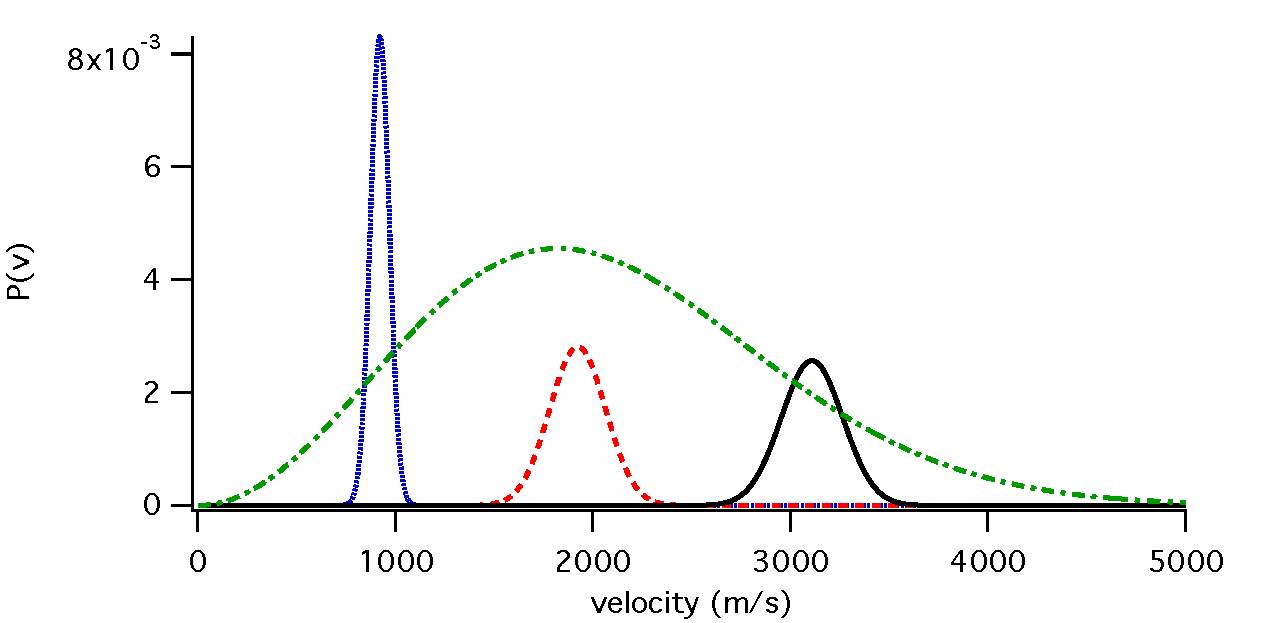
\includegraphics[width=1.0\textwidth]{Figures/diffractionPofv2.pdf}}
\caption[Probability distribution of velocities in supersonic atom beams.]{\label{diffractionPofv} Probability distribution of velocities for supersonic beams of Rb (blue dotted), K (red dashed), and Na (black solid), as measured in Figure \ref{nakrbDiffraction}. Each distribution is normalized such that $\int_0^\infty P(v) dv =1$. For comparison, we also show the velocity distribution of a Maxwell-Boltzmann gas of He atoms at 800 K (green dot-dashed) that is used as the carrier gas for the Na supersonic beam, normalized to 10 for visibility.}
\end{figure}






